\chapter{Graph Theory}

\section{Definitions}

A graph can be represented as the pair $G(V, E)$ where $V$
is the set of \textit{vertices}, and $E$ is the set of
\textit{edges}. Each element in $E$ is an unordered pair of
the vertices connected by the edge.

$$V = \{a, b, c, d\}$$
$$E = \{(a, b), (a, c), (b, c), (c, d)\}$$

\begin{center}
    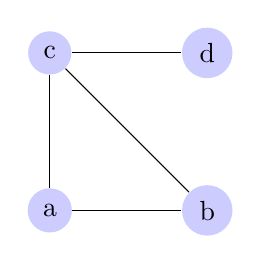
\begin{tikzpicture}[scale=2,every node/.style={circle,fill=blue!20}]
        \node (n1) at (1, 1) {a};
        \node (n2) at (2, 1) {b};
        \node (n3) at (1, 2) {c};
        \node (n4) at (2, 2) {d};

        \draw (n1) -- (n2);
        \draw (n1) -- (n3);
        \draw (n2) -- (n3);
        \draw (n3) -- (n4);
    \end{tikzpicture}
\end{center}

\begin{description}
    \item[Order] The number of vertices in a graph is the
    \textit{order}, or $|V|$.

    \item[Size] The number of edges in a graph is the
    \textit{size}, or $|E|$.

    \item[Degree] The number of edges incident to a vertex
    is the \textit{degree} of the vertex.

\end{description}

\section{Simple Graphs}

\begin{description}
    \item[Theorem] The sum of all degrees of $G$ equals
    twice the size of $G$.

    \item[Theorem] The sum of all degrees of $G$ must be
    even.

    \item[Regular Graph] A graph where all vertices have
    the same degree.

    \item[Complete Graph] A graph where all vertices are
    connected. The complete graph of order $n$ is denoted
    by $K_n$.
    
    \begin{center}
        \begin{tikzpicture}[scale=2,every node/.style={circle,fill=blue!20}]
            \graph { subgraph K_n [n=5,clockwise,radius=2cm] };
        \end{tikzpicture}

        Above, $K_5$ is shown.
    \end{center}
\end{description}

\section{Isomorphic Graphics}

Two graphs are isomorphic if they are the ''same''. More
formally, the graphs are isomorphic if there exists a
one-to-one correspondance between the vertices of each
graph.

Some properties of isomorphic graphs:
\begin{itemize}
    \item Same order
    \item Same size
    \item Same degrees
\end{itemize}

\section{Connected Graphs \& Walks}

\begin{description}
    \item[Walk] Any ordering of vertices each connected by
    an edge.

    \item[Connected] A graph is connected if it is possible
    to create a walk between any two vertices.

    \item[Trail] A walk with no repeated edges

    \item[Path] A walk with no repeated vertices

    \item[Circuit] A trail which starts \& ends at the same
    vertex.

    \item[Cycle] A circuit with no repeated vertices
    (except starting \& ending vertices).

    \begin{description}
        \item[Theorem] A cycle can be constructed from
        any circuit

        \item[Proof] In the case that the circuit doesn't
        have any repeated vertices, it is already a cycle.
        In the other case, represent the circuit as
        $v_i - ... - v_k - ... - v_k - ... - v_f$. Replace
        $v_k - ... - v_k$ with $v_k$ to remove the repetition.
    \end{description}

    \item[Euler circuit] A circuit that contains all the
    edges of the graph.

    \item[Traversable] A trail that contains all edges but
    starts \& ends at different vertices.

    \item[Hamiltonian Cycle] A path that visits each vertex
    exactly once and starts \& ends at the same vertex.

    Properties of Hamiltonian Graphs
    \begin{itemize}
        \item Connected
        \item All degrees are $> 1$
    \end{itemize}

    For a graph with order $n > 2$, if each degree is
    $\geq \frac{p}{2}$, it must be Hamiltonian.
\end{description}
